\section{Discriminative Topic Model with Block Prior and Various Features}
\label{sec:model}

Our model is able to identify blocks from the network with an embedded
\wsbm, extract topic patterns of each block as prior knowledge, and
use all this information to reconstruct the links.

\subsection{\lda with Block Priors (\bplda)}
\label{ssec:gen_doc}

\begin{figure}[t!]
  \centering
  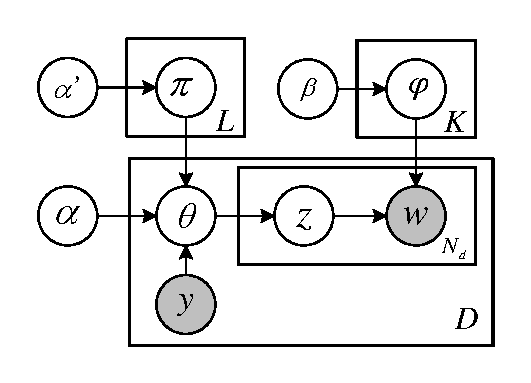
\includegraphics[width=.6\linewidth]{2016_acl_docblock/figures/wsbtm.pdf}
  \caption{Graphical Model of \bplda}\label{fig:wsbtm}
\end{figure}

As argued in the introduction, linked documents are likely to have
similar topic distributions, which can be generalized to documents in
the same block.  Inspired by this intuition and the block assignment
we obtain in the previous section, we want to extract some prior
knowledge from these blocks.  Thus we propose an \lda with \underline{b}lock \underline{p}riors, hence \bplda, as shown in
Figure~\ref{fig:wsbtm}, which has the following generative process:\par\nobreak
\begin{small}
\begin{enumerate}[leftmargin=*,noitemsep]
\item For each topic $k \in \{1,\ldots,K\}$
    \begin{enumerate}
    \item Draw word distribution $\bm{\phi_k} \sim \mathrm{Dir}(\beta)$
    \end{enumerate}
\item For each block $l\in \{1,\ldots,L\}$
    \begin{enumerate}
    \item Draw topic distribution $\bm{\pi_l}\sim \mathrm{Dir}(\alpha')$
    \end{enumerate}
\item For each document $d\in \{1,\ldots,D\}$
    \begin{enumerate}
    \item Draw topic distribution $\bm{\theta_d}\sim \mathrm{Dir}(\alpha \bm{\pi_{y_d}})$
    \item For each token $t_{d,n}$ in document $d$
        \begin{enumerate}
        \item Draw topic assignment $z_{d,n}\sim \mathrm{Mult}(\bm{\theta_d})$
        \item Draw word $w_{d,n}\sim \mathrm{Mult}(\bm{\phi_{z_{d,n}}})$
        \end{enumerate}
    \end{enumerate}
\end{enumerate}
\end{small}

Unlike conventional \lda, which uses an uninformative topic prior, \bplda puts a
Dirichlet prior~$\bm{\pi}$ on each block to capture the block's topic
distribution and use it as an informative prior when drawing each document's
topic distribution.  In other words, a document's topic distribution---i.e.,
what the document is about---is not just informed by the words present in the
document but the broader context of its network neighborhood.

\subsection{\rtm with Various Features (\vfrtm)}
\label{ssec:gen_links}

Building on~\newcite{chang-2010-rtm}, we want to generate the links
between documents based on \underline{v}arious \underline{f}eatures,
hence \vfrtm.  In addition to topic distributions, \vfrtm also
includes documents' word distributions~\cite{nguyen-2013-lexical} and
the link rate of two documents' assigned blocks, with the intent that
these additional features improve link generation.  \vfrtm involves
the relationship between a pair of documents, so it is difficult to
show the whole model; therefore Figure~\ref{fig:lex_block_rtm}
illustrates with a two-document segment.

\begin{figure}[t!]
  \centering
  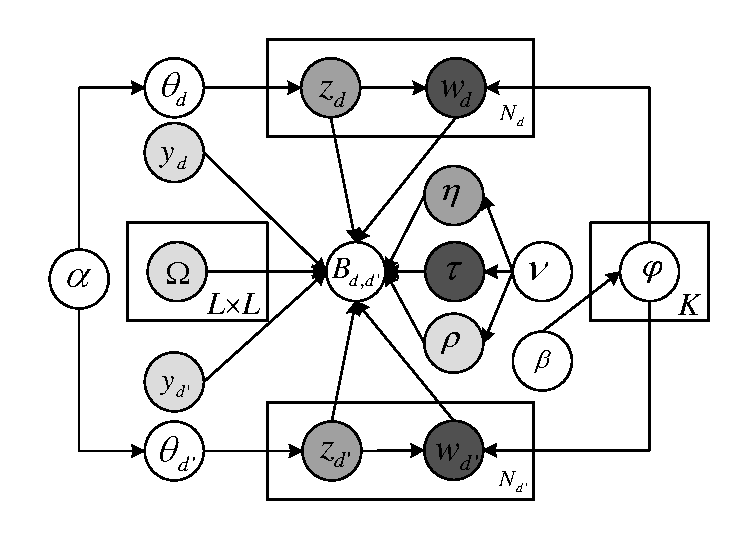
\includegraphics[width=.8\linewidth]{2016_acl_docblock/figures/lex_block_rtm.pdf}
  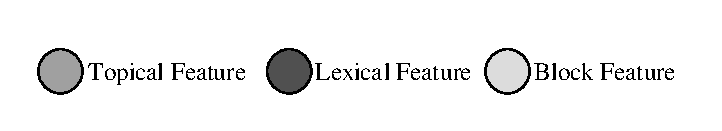
\includegraphics[width=\linewidth]{2016_acl_docblock/figures/lex_block_rtm_legend.pdf}
  \caption{A two-document segment of \vfrtm. Various features are
    denoted by grayscale.~$B_{d,d'}$ is observed, but we keep it in
    white background to avoid confusion.}\label{fig:lex_block_rtm}
  
\end{figure}

\noindent The generative process is:

\begin{small}
\begin{enumerate}[leftmargin=*,noitemsep]
\item For each pair of blocks $(l,l')\in \{1,\ldots,L\}^2$
    \begin{enumerate}
    \item Draw block regression parameter $\rho_{l,l'}\sim \mathcal{N}(0,\nu^2)$
    \end{enumerate}
\item For each topic $k\in \{1,\ldots,K\}$
    \begin{enumerate}
    \item Draw word distribution $\bm{\phi_k}\sim \mathrm{Dir}(\beta)$
    \item Draw topic regression parameter $\eta_k\sim \mathcal{N}(0,\nu^2)$
    \end{enumerate}
\item For each word $v\in \{1,\ldots,V\}$
    \begin{enumerate}
    \item Draw lexical regression parameter $\tau_v\sim \mathcal{N}(0,\nu^2)$
    \end{enumerate}
\item For each document $d\in \{1,\ldots,D\}$
    \begin{enumerate}
    \item Draw topic distribution $\bm{\theta_d}\sim \mathrm{Dir}(\alpha)$
    \item For each token $t_{d,n}$ in document $d$
        \begin{enumerate}
        \item Draw topic assignment $z_{d,n}\sim \mathrm{Mult}(\bm{\theta_d})$
        \item Draw word $w_{d,n}\sim \mathrm{Mult}(\bm{\phi_{z_{d,n}}})$
        \end{enumerate}
    \end{enumerate}
\item For each explicit link $(d,d')$
    \begin{enumerate}
    \item Draw link weight\\
    $B_{d,d'}\sim \Psi(\cdot\,|\,y_d, y_{d'}, \bm{\Omega}, \bm{z_d}, \bm{z_{d'}}, \bm{w_d}, \bm{w_{d'}}, \bm{\eta}, \bm{\tau}, \bm{\rho})$
    \end{enumerate}
\end{enumerate}
\end{small}

Links are generated by a link probability function~$\Psi$ which
takes the regression value~$R_{d,d'}$ of documents~$d$ and~$d'$ as
an argument.  Assuming documents $d$ and $d'$ belong to blocks~$l$ and~$l'$
respectively,~$R_{d,d'}$ is
\begin{equation}\label{equ:regression}
\small
R_{d,d'} = \bm{\eta}^\mathrm{T} (\overline{\bm{z}}_d \circ \overline{\bm{z}}_{d'}) + \bm{\tau}^\mathrm{T} (\overline{\bm{w}}_d \circ \overline{\bm{w}}_{d'}) + \rho_{l, l'} \Omega_{l, l'},
\end{equation}
where~$\overline{\bm{z}}_d$ is a $K$-length vector with each element~$\overline{z}_{d,k} = \frac{1}{N_d} \sum_{n} \ind{z_{d,n} = k}$;~$\overline{\bm{w}}_d$ is a $V$-length vector with each element~$\overline{w}_{d,v} = \frac{1}{N_d} \sum_{n} \ind{w_{d,n} = v}$;~$\circ$ denotes the Hadamard (element-wise) product;\footnote{As~\newcite{chang-2010-rtm} point out, the Hadamard product is able to capture similarity between hidden topic representations of two documents.}~$\bm{\eta}$,~$\bm{\tau}$, and~$\bm{\rho}$ are the weight vectors and matrix for topic-based,
lexical-based and rate-based predictions, respectively.

A common choice of~$\Psi$ is a sigmoid~\cite{chang-2010-rtm}.
However, we instead use hinge loss so that \vfrtm can use the
max-margin principle, making more effective use of side information
when inferring topic assignments~\cite{zhu-2012-medlda}.  Using hinge
loss, the probability that documents~$d$ and~$d'$ are linked is
\begin{equation}\label{equ:psi_hinge}
\small
\Pr \bigbrack{B_{d,d'}} = \exp \bigbrack{-2 \max (0, \zeta_{d,d'})},
\end{equation}
where~$\zeta_{d,d'} = 1 - B_{d,d'} R_{d,d'}$. Positive and negative
link weights are denoted by 1 and -1, respectively, in contrast to
sigmoid loss.

\subsection{Aggregated Model}
\label{ssec:lex_wsb_rtm}

\begin{figure*}[th]
  \centering
  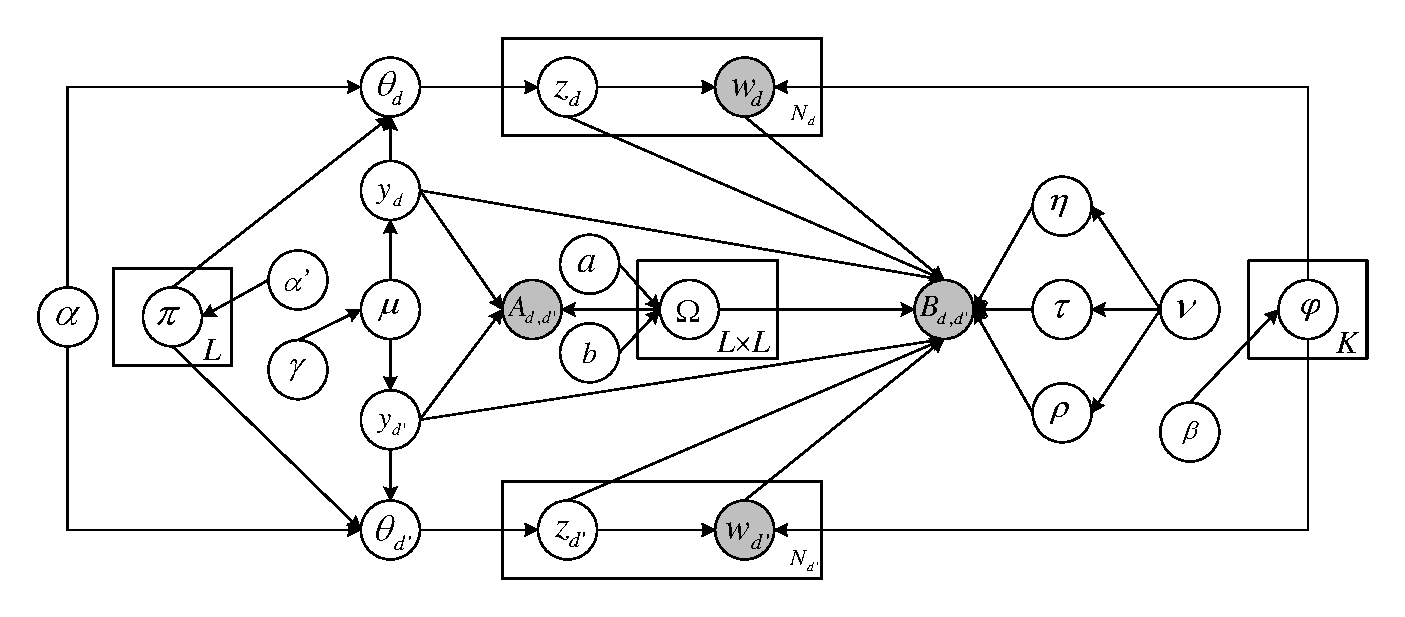
\includegraphics[width=.85\linewidth]{2016_acl_docblock/figures/lex_wsb_rtm.pdf}
  \caption{The graphical model of \lexwsbmedrtm for two documents, in
    which a weighted stochastic block model is embedded ($\gamma$,
    $\mu$, $y$, $a$, $b$, $\bm{\Omega}$, and~$\bm{A}$). Each document's
    topic distribution has an informative prior~$\bm{\pi}$. The model
    predicts links between documents ($\bm{B}$) based on topics
    ($\bm{z}$), words ($\bm{w})$, and inter-block link rates
    ($\bm{\Omega}$), using a max-margin
    objective.}\label{fig:graphical_model}
\end{figure*}

Finally, we put all the pieces together and propose \lexwsbmedrtm:
\rtm with lexical weights (\lex), block priors (\wsb), and hinge loss
(\med). Its graphical model is given in
Figure~\ref{fig:graphical_model}.




\begin{small}
\begin{enumerate}[leftmargin=*,noitemsep]
\item For each pair of blocks $(l,l')\in \{1,\ldots,L\}^2$
    \begin{enumerate}
    \item Draw inter-block link rate $\Omega_{l,l'}\sim \mathrm{Gamma}(a,b)$
    \item Draw block regression parameter $\rho_{l,l'}\sim \mathcal{N}(0,\nu^2)$
    \end{enumerate}
\item Draw block distribution $\bm{\mu}\sim \mathrm{Dir}(\gamma)$
\item For each block $l\in \{1,\ldots,L\}$
    \begin{enumerate}
    \item Draw topic distribution $\bm{\pi_l}\sim \mathrm{Dir}(\alpha')$
    \end{enumerate}
\item For each topic $k\in \{1,\ldots,K\}$
    \begin{enumerate}
    \item Draw word distribution $\bm{\phi_k}\sim \mathrm{Dir}(\beta)$
    \item Draw topic regression parameter $\eta_k\sim \mathcal{N}(0,\nu^2)$
    \end{enumerate}
\item For each word $v\in \{1,\ldots,V\}$
    \begin{enumerate}
    \item Draw lexical regression parameter $\tau_v\sim \mathcal{N}(0,\nu^2)$
    \end{enumerate}
\item For each document $d\in \{1,\ldots,D\}$
    \begin{enumerate}
    \item Draw block assignment $y_d\sim \mathrm{Mult}(\bm{\mu})$
    \item Draw topic distribution $\bm{\theta_d}\sim \mathrm{Dir}(\alpha \bm{\pi_{y_d}})$
    \item For each token $t_{d,n}$ in document $d$
        \begin{enumerate}
        \item Draw topic assignment $z_{d,n}\sim \mathrm{Mult}(\bm{\theta_d})$
        \item Draw word $w_{d,n}\sim \mathrm{Mult}(\bm{\phi_{z_{d,n}}})$
        \end{enumerate}
    \end{enumerate}
\item For each link $(d,d') \in \{1,\ldots,D\}^2$
    \begin{enumerate}
    \item Draw link weight $A_{d,d'} \sim \mathrm{Poisson} (\Omega_{y_d,y_{d'}})$
    \end{enumerate}
\item For each explicit link $(d,d')$
    \begin{enumerate}
    \item Draw link weight\\
    $B_{d,d'}\sim \Psi(\cdot\,|\,y_d, y_{d'}, \bm{\Omega}, \bm{z_d}, \bm{z_{d'}}, \bm{w_d}, \bm{w_{d'}}, \bm{\eta}, \bm{\tau}, \bm{\rho})$
    \end{enumerate}
\end{enumerate}
\end{small}

$\bm{A}$ and~$\bm{B}$ are assumed independent in the model,
but they can be derived from the same set of links in practice.

Link set~$\bm{A}$ is primarily used to find blocks, so it treats all
links \emph{deterministically}.  In other words, the links observed in the
input are considered explicit positive links, while the unobserved
links are considered explicit negative links, in contrast to the
implicit links in~$\bm{B}$.

In terms of link set~$\bm{B}$, while it adopts all explicit positive
links from the input, it \emph{does not deny} the existence of unobserved
links, or implicit negative links. Thus~$\bm{B}$ consists of only
explicit positive links. However, to avoid overfitting, we
sample some implicit links and add them to~$\bm{B}$ as explicit
negative links.